\chapter{The Large Hadron Collider}

\section{scratch section to work out outline...}
First thing to do is introduce the LHC as the large hadron collider and mention where it is located.  Now I should give a brief overview of what it does.  Now I need to talk about how it does this.  That means I need to mention how the protons are accelerated.  Then I need to explain how we contain and collide them once they are accelerated.  This leads into talking about the tunnel and magnets used for steering the bunches.

\section{Introduction}
The Large Hadron Collider (LHC) is a 26.7 kilometer-long two-ring particle accelerator and collider located on the border of France and Switzerland at the European Organization for Nuclear Research (CERN).  During normal operations the LHC maintains two counter-rotating beams of proton bunches that collide at four interaction points (IP).  The ALICE (Point 2), ATLAS (Point 1), CMS (Point 5), and LHC-b experiments each have a detector at one of these interaction points as scene in Figure \ref{fig:lhcips} .  The CMS and ATLAS are general-purpose detectors while LHC-b specializes in beauty quark studies.  ALICE is a heavy-ion experiment which uses $^{208}Pb-p$ or $^{208}Pb-^{208}Pb$ collisions that can also be produced by the LHC.

\begin{figure}[h]
	\centering
	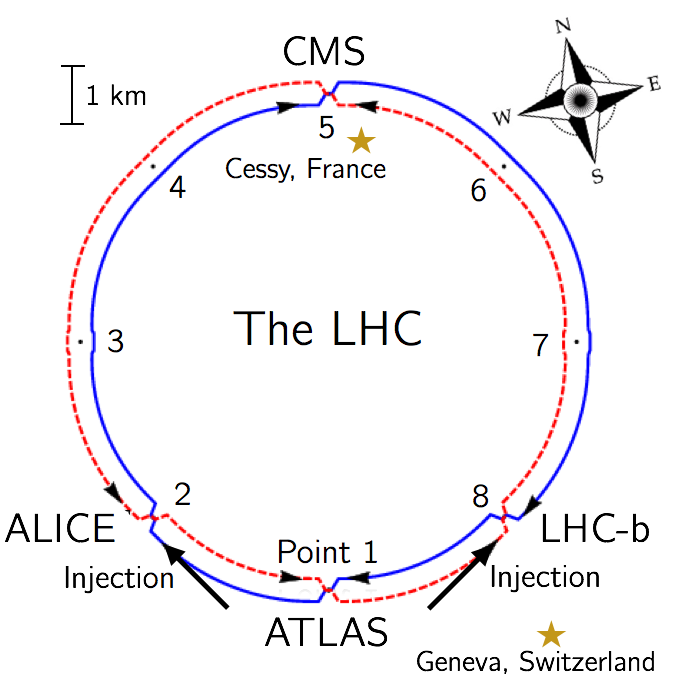
\includegraphics[width=0.7\linewidth]{Figures/LHC_IPs}
	\caption[LHC interaction points]{Interaction points of the LHC}
	\label{fig:lhcips}
\end{figure}


\section{Injector Chain}


\section{Tunnel and Magnets}


\section{Luminosity} 
